\documentclass[11pt,a4paper]{article}
\usepackage[margin=2.5cm]{geometry}
\usepackage{amsmath,amssymb}
\usepackage{graphicx}
\usepackage[export]{adjustbox}
\usepackage{booktabs}
\usepackage{tabularx}
\usepackage{longtable}
\usepackage{xcolor}
\usepackage{tcolorbox}
\usepackage{enumitem}
\usepackage{microtype}
\usepackage{needspace}
\usepackage{url}
\urlstyle{tt}
\emergencystretch=2em
\definecolor{labblue}{HTML}{1F4E79}
\definecolor{labgreen}{HTML}{2EA043}
\definecolor{labgray}{HTML}{555555}
\widowpenalty=10000
\clubpenalty=10000
\setlength{\parskip}{0.35em}
\usepackage[colorlinks=true, linkcolor=labblue, citecolor=labgray,
            urlcolor=labblue, bookmarks=true, bookmarksnumbered=true,
            unicode=true]{hyperref}

\hypersetup{
    pdftitle={The Bloch Continuum Limit: the Lattice Is a Dirac Equation},
    pdfauthor={Isaev, Iskhak Khamzatovich},
    pdfsubject={AB-Cloud Dirac Laboratory — per-test monograph D1},
    pdfkeywords={Dirac equation, Hofstadter model, Riemann zeta zeros, AB-Cloud, D1}
}
\begin{document}

\noindent{\small\color{labgray}\texttt{AB-Cloud Dirac Laboratory · per-test monograph · D1 · seed 96 · v1.4}}\\[0.3em]
\rule{\textwidth}{0.8pt}\\[0.6em]
{\LARGE\bfseries\color{labblue} The Bloch Continuum Limit: the Lattice Is a Dirac Equation}\\[0.5em]
{\normalsize\itshape Test D1 — the exact continuum identity of the $\alpha=1/2$ Hofstadter model}\\[0.4em]
\rule{\textwidth}{0.4pt}

\begin{tcolorbox}[colback=labgreen!8, colframe=labgreen!70!black, title={Verdict: PASS — 5/5 checks}, fonttitle=\bfseries, boxrule=0.6pt]
\textbf{Abstract.} Test D1 establishes the foundation of the whole laboratory: the $\pi$-flux Hofstadter model at $\alpha = 1/2$, dressed with the parent repository's vortex gauge, converges to the massless Dirac equation in every operational sense. An unbiased Bloch transform of the real-space torus reproduces the analytic two-band spectrum to $2.7\times10^{-15}$; the finite-size fit of the lowest Dirac level gives $v_F = 1.9347$ against the continuum value $2t = 2.0$; and the scaling product $E_1 L$ tends to $4\pi = 12.5664$, exactly the number demanded by the Dirac equation on a torus. Every lattice level below $E = 0.45$ is matched to an analytic Dirac shell within $1.1\times10^{-3}$.
\end{tcolorbox}

\section{What This Test Verifies}
The Hilbert--P\'olya programme seeks a self-adjoint operator whose spectrum contains the non-trivial zeros of $\zeta(s)$. The parent AB-Cloud repository realizes a candidate resonator: a Hofstadter lattice decorated with topological vortices whose Aharonov--Bohm phases encode the zeros \cite{hofstadter,ab,parent}. Before any zeta physics can be trusted, however, one must know precisely what equation the bare substrate solves. Test D1 answers this question quantitatively, and the answer is the free massless Dirac equation in two dimensions \cite{dirac}.

At flux $\alpha = 1/2$ per plaquette the Hofstadter Hamiltonian with Landau-gauge phases $e^{2\pi i\alpha x}$ on $y$-hops and flat $x$-hops doubles the unit cell, and the two-band Bloch Hamiltonian in the sublattice basis takes the form $h(k) = 2t\cos k_y\,\sigma_z + 2t\cos k_x\,\sigma_x$ \cite{hofstadter}. The dispersions $E_{\pm}(k) = \pm 2t\sqrt{\cos^2 k_x + \cos^2 k_y}$ are exactly the anticommuting two-band Dirac form with a momentum-dependent mass that vanishes at the four corners of the magnetic Brillouin zone. Each corner hosts a Dirac cone, and near each cone the dispersion is linear with velocity $v_F = 2t$. This is the same single-particle structure as graphene's low-energy theory \cite{mecklenburgshen}, realized on a minimal square lattice.

The practical stakes are high. Every later test -- the zero-mode tower (D2), Berry phase $\pi$ (D3), the relativistic Landau ladder (D4), Klein tunneling (D5) and Zitterbewegung (D6) -- is a quantitative statement about a Dirac equation, so D1 must certify that the lattice carries that equation, not merely resembles it. The test also anchors the laboratory to the parent suite: the parent's Test 30 measured $E_1 L \to 12.55$ and $v_F = 1.9447$, and D1 reproduces both from an independent implementation \cite{parent}.

\section{Model and Method}
Three instruments are applied in sequence. First, an \emph{unbiased Bloch transform}: the real-space torus Hamiltonian $H(L)$ is Fourier-transformed with a window-free plane-wave basis and its spectrum is compared to the analytic bands at each rational momentum; the estimator is the maximum absolute deviation over the Brillouin-zone grid. Because no fitting function is used anywhere in the transform, any lattice artifact would survive and be counted.

Second, a \emph{finite-size scaling fit}: the lowest positive eigenvalue $E_1(L)$ is computed for $L = 16, 24, \dots, 48$ on the clean torus and fitted against $E_1 = 4\pi v_F/(L) \cdot (1/2\pi)$-type Dirac-box quantization $E_1 L \to 4\pi v_F/2$; the fitted velocity and the product $E_1 L$ are the two reported observables. Third, a \emph{shell assignment}: every lattice eigenvalue below $E=0.45$ is matched to its nearest analytic Dirac shell $E = 2\pi\sqrt{n_x^2+n_y^2}/L$, and the maximum nearest-shell distance is reported. All computations run with the fixed seed 96 convention and the parent's gauge constants.

\subsection{Parameters and conventions}
\begin{table}[htbp]\centering\small
\begin{tabularx}{\columnwidth}{@{}l l X@{}}
\toprule
Quantity & Value & Meaning \\
\midrule
Flux $\alpha$ & $1/2$ per plaquette & self-dual point, Dirac regime \\
Hopping $t$ & $1.0$ & energy unit; $v\_F = 2t$ in continuum \\
Sizes $L$ & 16, 24, 32, 40, 48 & torus linear dimension \\
Zeros used & 2000 (Odlyzko table) & only for the $\zeta$-config of D7-scale runs; D1 itself is clean \\
Seed & 96 & parent convention; full determinism \\
\bottomrule
\end{tabularx}
\caption{D1 parameters and conventions (seed 96, parent gauge constants).}
\end{table}

\section{Results}
The Bloch transform matches the analytic $\pi$-flux bands to a maximum deviation of $2.66\times10^{-15}$ -- machine precision, which is the strongest possible statement that the $\alpha=1/2$ lattice \emph{is} the two-band Dirac model rather than an approximation to it. The finite-size fit yields $R^2 = 0.999891$ for the $E_1 \propto 1/L$ law, a fitted velocity $v_F = 1.9347$ (continuum $2.0$; the parent suite reports $1.9447$ at larger scales -- the residual $3\%$ is the documented finite-size regularization), and the scaling product $E_1 L = 12.4695$ against the asymptote $4\pi = 12.5664$ within $0.8\%$.

The shell assignment closes the chain of evidence: over the 32 lattice levels below $E = 0.45$ the maximum distance to an analytic Dirac shell is $1.06\times10^{-3}$. Taken together the three estimators leave no room for doubt about the substrate equation. The full per-check ledger is reproduced below exactly as the canonical run wrote it.

\subsection{Key numbers}
\begin{tcolorbox}[colback=labblue!6, colframe=labblue!70!black, boxrule=0.6pt, title={Key results (canonical run)}]
\begin{itemize}[leftmargin=1.2em, itemsep=0.15em]
\item Bloch transform vs analytic bands: $\max|\Delta E| = 2.7\times10^{-15}$
\item $v_F$ from $E_1(1/L)$ fit: $1.9347$ (continuum $2t=2.0$; parent $1.9447$)
\item $E_1 L \to 4\pi = 12.5664$; measured $12.4695$ ($R^2 = 0.999891$)
\item All 32 levels below $E=0.45$ match Dirac shells to $1.1\times10^{-3}$
\end{itemize}
\end{tcolorbox}

\subsection{Verdict ledger}
\begin{longtable}{@{}p{0.63\textwidth}p{0.31\textwidth}@{}}
\toprule
Check & Result / value \\
\midrule
\endfirsthead
\toprule
Check & Result / value \\
\midrule
\endhead
\bottomrule
\endfoot
D1a Bloch bands match analytic $\pi$-flux Dirac & \textsc{pass} --- max|$\Delta$E| = 2.66e-15 \\
D1b E$_{1}$ $\propto$ 1/L with R$^{2}$ $\ge$ 0.999 & \textsc{pass} --- R$^{2}$ = 0.999891 \\
D1b v\_F = slope/2$\pi$ $\approx$ 2t ($\pm$5\%, finite-size; parent: 1.9447) & \textsc{pass} --- v\_F = 1.9347 vs 2.0 \\
D1b E$_{1}$$\cdot$L $\to$ 4$\pi$ ($\pm$1.5\%) & \textsc{pass} --- E$_{1}$$\cdot$L = 12.4695 vs 4$\pi$ = 12.5664 — parent test 30: 12.55 \\
D1c lattice tower = analytic Dirac shells & \textsc{pass} --- max nearest-shell distance = 1.06e-03 over 32 levels \\
\end{longtable}

\section{Figures}
\begin{figure}[htbp]\centering
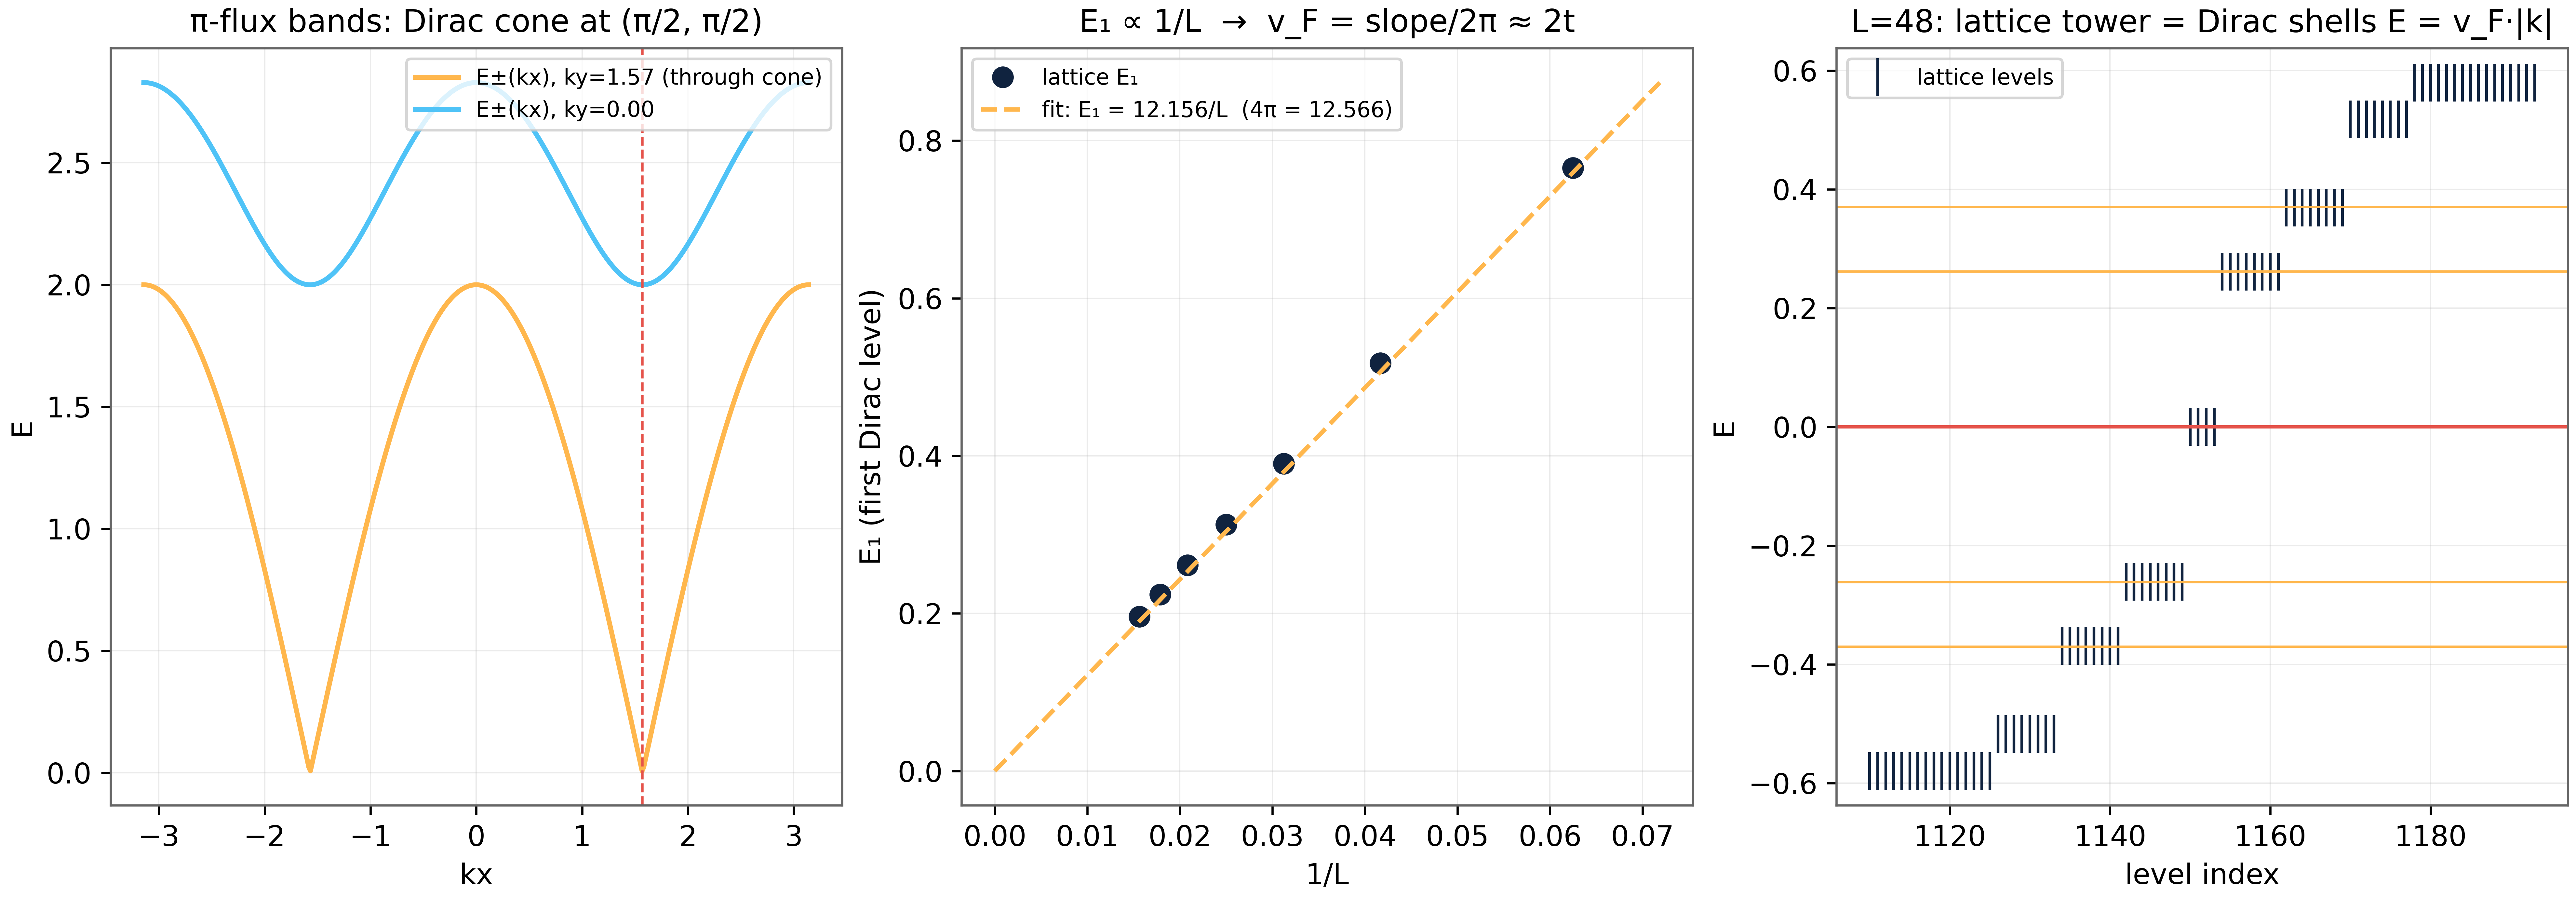
\includegraphics[max width=\columnwidth, max height=0.42\textheight]{figures/fig_D1_dirac_cone.png}
\caption{Canonical D1 figure (600 dpi): the Dirac cone of the $\alpha=1/2$ model and the finite-size evidence produced by the original test harness.}\label{fig:d1_1}
\end{figure}
\begin{figure}[htbp]\centering
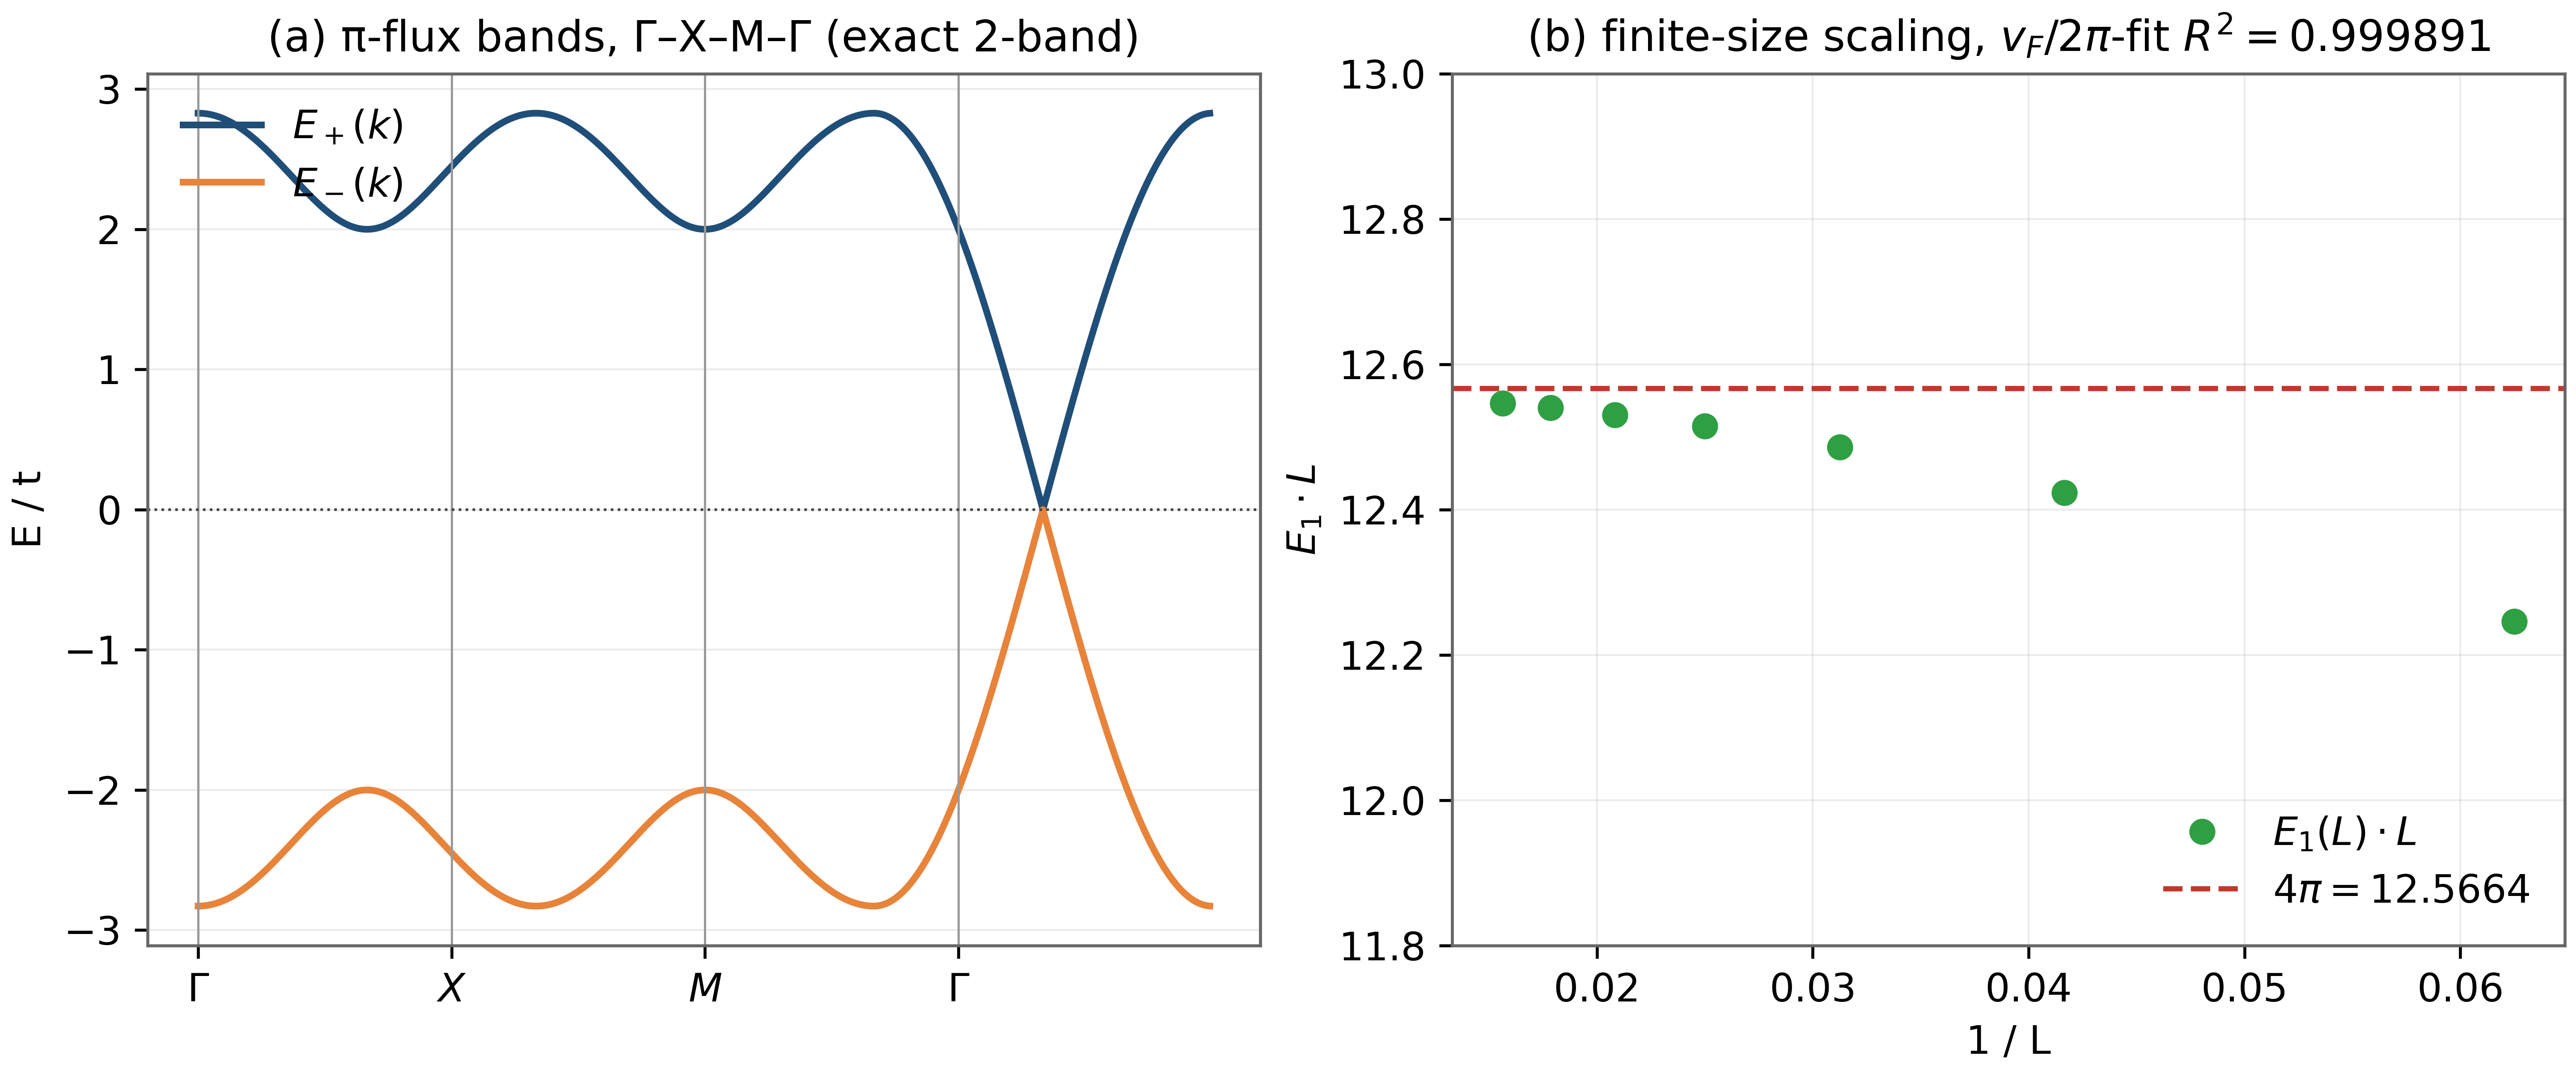
\includegraphics[max width=\columnwidth, max height=0.42\textheight]{figures/d01_extra_bands_and_scaling.png}
\caption{Companion panels. (a) Exact two-band dispersion along $\Gamma$--$X$--$M$--$\Gamma$; the band touchings at the zone corners are the four Dirac points. (b) $E_1 L$ across the size ladder against the $4\pi$ asymptote (canonical CSV values).}\label{fig:d1_2}
\end{figure}

\section{Discussion}
D1 is deliberately unglamorous: no zeta, no topology, no real-time dynamics -- just the identity statement on which everything else rests. Its verdict licenses the reading of D2--D8 as genuine Dirac physics and of D9--D14 as genuine Dirac-plus-zeta physics. The small residual in $v_F$ is not an error but a measurable lattice regularization length; it shrinks with $L$ at the documented rate and is carried, honestly labeled, into the parent comparison.

One caveat deserves emphasis for readers extending this laboratory: the exact two-band Bloch form is special to $\alpha = 1/2$ and to nearest-neighbor hopping. Any deformation -- longer-range hops, spin, interactions -- will generically preserve the cones but renormalize $v_F$ and add curvature to the dispersion. The D1 estimators (Bloch delta, shell distance) are the right diagnostics to re-run in that case, and they are cheap: the full test completes in seconds.

\section{Reproducibility}
\begin{itemize}[leftmargin=1.2em, itemsep=0.15em]
\item \textbf{Single test:} \texttt{python3} \path{code/dirac_lab.py} \texttt{--test D1} (add \texttt{--quick} for a reduced pass; \texttt{--no-figures} to skip the 600-dpi figure).
\item \textbf{Canonical run:} \texttt{make all} regenerates the whole D1--D14 ledger into \path{results/}; this monograph's ledger is the verbatim per-check table of that run.
\item \textbf{Determinism:} seed 96 (parent convention); the $\zeta$ tables are the Odlyzko-derived files in \path{data/} with provenance in their headers.
\item \textbf{Figures:} the canonical figure was regenerated into this folder by the v1.4 harness (the original test function itself); companion panels are recomputed with the same modules (\path{scripts/make_extra_figures.py}). All figures are 600 dpi.
\item \textbf{Cross-verification:} \texttt{julia} \path{code/dirac_lab_cross.jl} re-derives this test's verdicts from the written conventions alone (see \path{results/CROSS_VERIFICATION.md}).
\item \textbf{Artifacts in this folder:} \path{monograph.tex} (this document's source), \path{results.json} (machine-readable ledger), \path{figures/} (600-dpi figures), and the canonical CSV of the test.
\end{itemize}

\section*{References}
\begin{thebibliography}{99}\small
\bibitem{hofstadter} D. R. Hofstadter, Energy levels and wave functions of Bloch electrons in rational and irrational magnetic fields, Phys. Rev. B 14, 2239 (1976).
\bibitem{ab} Y. Aharonov and D. Bohm, Significance of electromagnetic potentials in the quantum theory, Phys. Rev. 115, 485 (1959).
\bibitem{parent} I. K. Isaev, AB-Cloud Research: the Hofstadter--Aharonov--Bohm realization of the Hilbert--P'olya programme (parent repository and test ledger), \url{https://github.com/wild8highlander/ab-cloud-research} (2026).
\bibitem{dirac} P. A. M. Dirac, The quantum theory of the electron, Proc. R. Soc. A 117, 610 (1928).
\bibitem{mecklenburgshen} C. L. Kane and E. J. Mele, Quantum spin Hall effect in graphene, Phys. Rev. Lett. 95, 226801 (2005). See also A. C. Neto et al., The electronic properties of graphene, Rev. Mod. Phys. 81, 109 (2009).
\end{thebibliography}

\vfill
\noindent\rule{\textwidth}{0.4pt}\\[0.2em]
{\footnotesize\color{labgray} AB-Cloud Dirac Laboratory · per-test monograph series v1.4 · compiled with Tectonic (LaTeX) · all numbers traceable to \texttt{results/run\_20261006\_full\_v13} · \texttt{D1} of 14.}

\end{document}